\chapter{The Hodge Conjecture}
\label{ch:hodge}

\medskip\noindent\textbf{Prerequisites.} This chapter assumes a solid background in linear algebra and some familiarity with basic topology, including the fundamental group and covering spaces. Some experience with complex analysis, particularly holomorphic functions and contour integration, will also be helpful. Differential forms and cohomology theory are developed from scratch within the chapter, so no prior knowledge of these topics is assumed.

\noindent\textbf{Key Ideas.}
\begin{itemize}
  \item The \emph{Hodge decomposition} splits cohomology of a K\"{a}hler manifold into types $(p,q)$.
  \item A \emph{Hodge class} is a rational cohomology class of type $(p,p)$.
  \item The Hodge conjecture says every Hodge class comes from algebraic cycles (subvarieties defined by polynomial equations).
  \item Known in codimension 1 (Lefschetz $(1,1)$ theorem), but open in higher codimensions.
\end{itemize}

\bigskip

\section{Introduction}

The Hodge conjecture is one of the seven Millennium Prize Problems, and it is the one most deeply rooted in algebraic geometry. At its heart, it asks a deceptively simple question: if a smooth projective variety---a space defined by polynomial equations in complex projective space---has a topological feature that is compatible with the complex structure in a precise sense, must that feature come from algebra? In other words, are the topological invariants of algebraic varieties entirely explained by their algebraic structure?

To make this more concrete, consider a smooth projective variety $X$ over $\mathbb{C}$, and consider its cohomology groups $H^{2p}(X, \mathbb{Q})$. These vector spaces measure the ``$2p$-dimensional holes'' of $X$---the topological features that cannot be deformed away. A subvariety $V \subseteq X$ of codimension $p$ defines a cohomology class $[V] \in H^{2p}(X, \mathbb{Q})$. This class records the ``shadow'' that $V$ casts in the topology of $X$. The Hodge conjecture asserts that every rational cohomology class of type $(p,p)$---a \emph{Hodge class}---is a linear combination of such shadows.

The conjecture was formulated by William Vallance Douglas Hodge in 1950, though Hodge himself described it more as a hope than a theorem. It is a bridge between two worlds: the world of topology (cohomology, Betti numbers, differential forms) and the world of algebra (polynomial equations, subvarieties, divisors). The conjecture predicts that this bridge is as short as possible---that every topological feature of algebraic origin is, in fact, of genuinely algebraic origin.

The difficulty lies in the word ``algebraic.'' It is easy to construct cohomology classes---just take any closed differential form and compute its cohomology class. But it is extremely hard to determine whether a given class is algebraic, i.e., whether it comes from an algebraic subvariety. The Hodge conjecture says that the only obstacle to a class being algebraic is the Hodge type: if the class is rational and has the right Hodge type $(p,p)$, then it is algebraic.

The conjecture is known in only a handful of cases. The Lefschetz $(1,1)$ theorem, proved in the 1920s, establishes it for codimension $p = 1$ (divisors). For curves and surfaces ($\dim X \le 2$), it holds trivially. But for higher-dimensional varieties, the conjecture is wide open in general. There are partial results for abelian varieties, K3 surfaces, and certain special classes of varieties, but no general proof. The integral version of the conjecture (with integer rather than rational coefficients) is false, as shown by Atiyah and Hirzebruch in 1962.

In this chapter, we develop the mathematical machinery needed to state the Hodge conjecture precisely and understand what is known. We begin with the complex geometry of projective space and algebraic varieties, move through de Rham cohomology and Hodge theory, introduce algebraic cycles and their cohomology classes, and culminate in a precise statement of the conjecture and a survey of what has been proved.

\section{Complex Manifolds and Projective Space}

\subsection{Complex Projective Space}

The stage for the Hodge conjecture is \emph{complex projective space}, the natural compactification of affine complex space.

\begin{definition}
\emph{Complex projective space} $\mathbb{P}^n(\mathbb{C})$ is the set of lines through the origin in $\mathbb{C}^{n+1}$. Equivalently, it is the quotient $(\mathbb{C}^{n+1} \setminus \{0\}) / \mathbb{C}^*$, where $\mathbb{C}^*$ acts by scalar multiplication.
\end{definition}

A point of $\mathbb{P}^n(\mathbb{C})$ is represented by \emph{homogeneous coordinates}
\[
[z_0 : z_1 : \cdots : z_n]
\]
where not all $z_i$ vanish, and $[z_0 : \cdots : z_n] = [\lambda z_0 : \cdots : \lambda z_n]$ for any $\lambda \in \mathbb{C}^*$. Two $n$-tuples that differ by a nonzero scalar represent the same point.

\begin{example}
$\mathbb{P}^1(\mathbb{C})$ is the Riemann sphere. A point $[z_0 : z_1]$ with $z_0 \neq 0$ can be written as $[1 : z_1/z_0]$, identified with the complex number $z = z_1/z_0$. The point $[0 : 1]$ corresponds to the point at infinity $\infty$. So $\mathbb{P}^1(\mathbb{C}) \cong \mathbb{C} \cup \{\infty\}$, which is topologically $S^2$.
\end{example}

\begin{example}
$\mathbb{P}^2(\mathbb{C})$ is the complex projective plane. It can be covered by three affine charts:
\[
U_i = \{[z_0 : z_1 : z_2] : z_i \neq 0\}, \qquad i = 0, 1, 2.
\]
On $U_0$, we use coordinates $(w_1, w_2) = (z_1/z_0, z_2/z_0)$, and the chart is isomorphic to $\mathbb{C}^2$. The complement $\mathbb{P}^2(\mathbb{C}) \setminus U_0$ is a copy of $\mathbb{P}^1(\mathbb{C})$, so $\mathbb{P}^2(\mathbb{C}) \cong \mathbb{C}^2 \cup \mathbb{P}^1(\mathbb{C})$.
\end{example}

More generally, $\mathbb{P}^n(\mathbb{C})$ is covered by $(n+1)$ affine charts $U_i \cong \mathbb{C}^n$, and can be written as
\[
\mathbb{P}^n(\mathbb{C}) = \mathbb{C}^n \cup \mathbb{P}^{n-1}(\mathbb{C}).
\]
As a real manifold, $\mathbb{P}^n(\mathbb{C})$ has real dimension $2n$. It is compact, connected, and orientable.

\subsection{Holomorphic Functions and Complex Manifolds}

A \emph{holomorphic function} $f: U \to \mathbb{C}$ on an open set $U \subseteq \mathbb{C}^n$ is a function that is complex-differentiable in each variable: for each $k$,
\[
\frac{\partial f}{\partial z_k} = \frac{1}{2}\left(\frac{\partial f}{\partial x_k} + i\, \frac{\partial f}{\partial y_k}\right)
\]
exists. Equivalently, $f$ is holomorphic if and only if it satisfies the Cauchy--Riemann equations $\partial f / \partial \bar{z}_k = 0$ for all $k$, where $\partial / \partial \bar{z}_k = \frac{1}{2}(\partial/\partial x_k + i\, \partial/\partial y_k)$.

\begin{definition}
A \emph{complex manifold} of dimension $n$ is a topological space $M$ (Hausdorff, second-countable) together with an atlas of charts $\{(U_\alpha, \phi_\alpha)\}$, where each $U_\alpha$ is open in $M$ and each $\phi_\alpha: U_\alpha \to \mathbb{C}^n$ is a homeomorphism onto an open subset of $\mathbb{C}^n$, such that the transition maps $\phi_\beta \circ \phi_\alpha^{-1}$ are holomorphic wherever defined.
\end{definition}

Complex projective space $\mathbb{P}^n(\mathbb{C})$ is a complex manifold: the transition maps between affine charts are
\[
\frac{z_j}{z_i} = \frac{z_j/z_k}{z_i/z_k},
\]
which are holomorphic rational functions (polynomials divided by nonzero polynomials).

\subsection{K\"{a}hler Metrics}

A \emph{K\"{a}hler metric} on a complex manifold is a Riemannian metric $g$ that is compatible with the complex structure $J$ and whose associated two-form $\omega$ (the K\"{a}hler form) is closed: $d\omega = 0$.

\begin{definition}
Let $(M, J)$ be a complex manifold with complex structure $J$ (a bundle endomorphism with $J^2 = -\mathrm{Id}$). A \emph{Hermitian metric} is a Riemannian metric $g$ such that $g(Jv, Jw) = g(v, w)$ for all tangent vectors $v, w$. The \emph{K\"{a}hler form} is the two-form $\omega(v, w) = g(Jv, w)$. The metric is \emph{K\"{a}hler} if $d\omega = 0$.
\end{definition}

The standard metric on $\mathbb{P}^n(\mathbb{C})$ is K\"{a}hler. On the affine chart $U_0 \cong \mathbb{C}^n$ with coordinates $(w_1, \ldots, w_n)$, the Fubini--Study metric is
\[
g = \frac{(1 + |w|^2)\,dw \cdot d\bar{w} - (\bar{w}\,dw)(w \cdot d\bar{w})}{(1 + |w|^2)^2}.
\]
Its K\"{a}hler form is
\[
\omega_{\text{FS}} = \frac{i}{2\pi} \partial\bar{\partial} \log(1 + |w|^2).
\]
The fact that $\omega_{\text{FS}}$ is closed ($d\omega_{\text{FS}} = 0$) follows from the identity $d = \partial + \bar{\partial}$ and $\partial^2 = \bar{\partial}^2 = 0$.

K\"{a}hler manifolds are the natural setting for the Hodge conjecture because they carry a rich interplay between topology, complex geometry, and harmonic analysis. Every smooth projective algebraic variety admits a K\"{a}hler metric (the restriction of the Fubini--Study metric), so the conjecture is formulated for these spaces.

\subsection{Examples of Complex Manifolds}

\begin{example}
The Riemann sphere $\mathbb{P}^1(\mathbb{C}) \cong S^2$ is a compact K\"{a}hler manifold of complex dimension 1 (real dimension 2). As a real manifold, it is topologically the 2-sphere.
\end{example}

\begin{example}
The complex projective plane $\mathbb{P}^2(\mathbb{C})$ is a compact K\"{a}hler manifold of complex dimension 2. Its real dimension is 4. Topologically, $\mathbb{P}^2(\mathbb{C})$ has Betti numbers $b_0 = 1$, $b_1 = 0$, $b_2 = 1$, $b_3 = 0$, $b_4 = 1$.
\end{example}

\begin{example}
A \emph{smooth hypersurface} $X_d \subset \mathbb{P}^n(\mathbb{C})$ of degree $d$ is defined by a single homogeneous polynomial equation $f(z_0, \ldots, z_n) = 0$ of degree $d$, where the gradient $\nabla f$ vanishes only at the origin. For example:
\begin{itemize}
\item $X_1 = \mathbb{P}^{n-1}(\mathbb{C})$ (a hyperplane), degree 1.
\item A smooth quadric $X_2 \subset \mathbb{P}^3(\mathbb{C})$ defined by $x^2 + y^2 + z^2 + w^2 = 0$, which is isomorphic to $\mathbb{P}^1(\mathbb{C}) \times \mathbb{P}^1(\mathbb{C})$.
\item The Fermat cubic surface $X_3 \subset \mathbb{P}^3(\mathbb{C})$ defined by $x^3 + y^3 + z^3 + w^3 = 0$, a smooth surface of general type.
\item The Fermat quintic threefold $X_5 \subset \mathbb{P}^4(\mathbb{C})$ defined by $x_0^5 + x_1^5 + x_2^5 + x_3^5 + x_4^5 = 0$, a Calabi--Yau threefold.
\end{itemize}
By the Lefschetz hyperplane theorem, a smooth hypersurface $X_d \subset \mathbb{P}^n(\mathbb{C})$ with $n \ge 2$ is connected, and its topology is largely controlled by the ambient projective space.
\end{example}

\begin{example}
An \emph{elliptic curve} is a smooth curve of genus 1. It can be realized as a smooth cubic in $\mathbb{P}^2(\mathbb{C})$, for example
\[
E: \quad y^2 z = x^3 + axz^2 + bz^3 \subset \mathbb{P}^2(\mathbb{C}).
\]
Topologically, an elliptic curve is a torus $T^2 = S^1 \times S^1$. It is a compact K\"{a}hler manifold of complex dimension 1.
\end{example}

\section{Algebraic Varieties}

\subsection{Projective Algebraic Varieties}

The objects studied in algebraic geometry are defined by polynomial equations.

\begin{definition}
A \emph{projective algebraic variety} $X \subseteq \mathbb{P}^N(\mathbb{C})$ is the zero set of a collection of homogeneous polynomials:
\[
X = \{[z_0 : \cdots : z_N] \in \mathbb{P}^N(\mathbb{C}) : f_1(z) = \cdots = f_k(z) = 0\}
\]
where each $f_i \in \mathbb{C}[z_0, \ldots, z_N]$ is homogeneous (all terms have the same degree). The variety is \emph{irreducible} if it cannot be written as $X = X_1 \cup X_2$ with $X_1, X_2$ proper subvarieties.
\end{definition}

The choice of homogeneous coordinates ensures that the zero set is well-defined: if $f$ is homogeneous of degree $d$, then $f(\lambda z) = \lambda^d f(z)$, so $f(z) = 0$ if and only if $f(\lambda z) = 0$ for $\lambda \neq 0$.

\begin{definition}
The \emph{dimension} of an irreducible variety $X$ is the dimension of $X$ as a complex manifold (at smooth points), or equivalently, the transcendence degree of the field of rational functions on $X$ over $\mathbb{C}$.
\end{definition}

\subsection{Smoothness and the Jacobian Criterion}

Not every point of an algebraic variety is a smooth point. Singularities occur where the variety fails to be a manifold.

\begin{definition}
A point $p \in X$ is \emph{smooth} (or \emph{nonsingular}) if the Jacobian matrix of the defining polynomials has rank equal to the codimension of $X$ at $p$. If every point of $X$ is smooth, we say $X$ is a \emph{smooth variety}.
\end{definition}

Concretely, if $X$ is a hypersurface defined by $f(z_0, \ldots, z_N) = 0$ in $\mathbb{P}^N(\mathbb{C})$, then $p \in X$ is smooth if and only if
\[
\left(\frac{\partial f}{\partial z_0}(p), \ldots, \frac{\partial f}{\partial z_N}(p)\right) \neq (0, \ldots, 0).
\]
For a variety defined by $k$ equations $f_1 = \cdots = f_k = 0$, the Jacobian matrix is $k \times (N+1)$, and smoothness at $p$ means this matrix has rank $k$ at $p$ (assuming $\operatorname{codim} X = k$).

\begin{example}
Consider the Fermat cubic curve $E: x^3 + y^3 + z^3 = 0$ in $\mathbb{P}^2(\mathbb{C})$. The gradient is
\[
\nabla f = (3x^2, 3y^2, 3z^2).
\]
This vanishes only at $[0 : 0 : 0]$, which is not a point of $\mathbb{P}^2(\mathbb{C})$. So $E$ is smooth.
\end{example}

\begin{example}
The curve $C: y^2 z = x^3$ in $\mathbb{P}^2(\mathbb{C})$ has a singularity at $[0 : 0 : 1]$, where $\nabla f = (-3x^2, 2yz, y^2) = (0, 0, 0)$. This is a cusp.
\end{example}

By a theorem of Bertini (in characteristic zero), a general hypersurface of degree $d \ge 1$ in $\mathbb{P}^n(\mathbb{C})$ (with $n \ge 1$) is smooth. So smooth varieties are ``generic'' rather than exceptional.

\subsection{Examples of Algebraic Varieties}

\begin{definition}
An \emph{elliptic curve} is a smooth projective curve of genus 1 with a marked point. Equivalently, it is a smooth cubic curve in $\mathbb{P}^2(\mathbb{C})$.
\end{definition}

An elliptic curve $E$ has complex dimension 1. Topologically it is a torus $T^2$, so its Betti numbers are $b_0 = 1$, $b_1 = 2$, $b_2 = 1$. The Hodge decomposition of $H^1(E, \mathbb{C})$ gives $H^{1,0}(E) \cong H^{0,1}(E) \cong \mathbb{C}$, so the Hodge diamond is
\[
\begin{array}{ccc}
 & 1 & \\
1 & & 1 \\
 & 1 &
\end{array}
\]
Elliptic curves are the simplest nontrivial examples for the Hodge conjecture, though the conjecture is trivially true for them (all Hodge classes are algebraic).

\begin{definition}
A \emph{K3 surface} is a smooth projective surface $X$ with $K_X \cong \mathcal{O}_X$ (trivial canonical bundle) and $H^1(X, \mathcal{O}_X) = 0$. Equivalently, it is a simply connected smooth projective surface with trivial canonical bundle.
\end{definition}

K3 surfaces are compact K\"{a}hler manifolds of complex dimension 2. Their Hodge diamond is
\[
\begin{array}{ccccc}
 & & 1 & & \\
 & 0 & & 0 & \\
1 & & 20 & & 1 \\
 & 0 & & 0 & \\
 & & 1 & &
\end{array}
\]
The Hodge conjecture for K3 surfaces is known: every Hodge class is algebraic. This was proved by Siu (1982) and others, building on work of van der Geer, Looijenga, and Piatetski-Shapiro.

\begin{definition}
A \emph{Calabi--Yau manifold} of complex dimension $n$ is a smooth projective variety with trivial canonical bundle ($K_X \cong \mathcal{O}_X$) and $H^i(X, \mathcal{O}_X) = 0$ for $0 < i < n$.
\end{definition}

The simplest Calabi--Yau manifolds are elliptic curves (dimension 1) and K3 surfaces (dimension 2). The most famous example in dimension 3 is the \emph{quintic threefold}: the smooth hypersurface $X_5 \subset \mathbb{P}^4(\mathbb{C})$ defined by
\[
x_0^5 + x_1^5 + x_2^5 + x_3^5 + x_4^5 = 0.
\]
The Hodge conjecture for Calabi--Yau threefolds is open in general. The quintic threefold has Hodge numbers $h^{1,1} = 1$ and $h^{2,1} = 101$, and the Hodge conjecture is known for it (by the Lefschetz $(1,1)$ theorem for divisor classes, and by other arguments for higher-codimensional classes).

\begin{definition}
An \emph{abelian variety} of dimension $g$ is a smooth projective variety that is isomorphic (as a complex Lie group) to a complex torus $\mathbb{C}^g / \Lambda$ for some lattice $\Lambda \cong \mathbb{Z}^{2g}$.
\end{definition}

Every abelian variety is a K\"{a}hler manifold. An elliptic curve is an abelian variety of dimension 1. Products of elliptic curves give higher-dimensional abelian varieties. The Hodge conjecture for abelian varieties is partially understood via the theory of Mumford--Tate groups, but is not known in general.

\section{De Rham Cohomology}

\subsection{Differential Forms}

To detect topological features of a manifold, we use differential forms.

\begin{definition}
On a smooth $n$-manifold $M$, a \emph{$k$-form} (or \emph{differential form of degree $k$}) is a smooth section of the bundle $\Lambda^k(T^*M)$ of alternating $k$-linear forms on tangent vectors. In local coordinates $(x_1, \ldots, x_n)$, a $k$-form can be written as
\[
\omega = \sum_{i_1 < \cdots < i_k} a_{i_1 \cdots i_k}(x)\, dx_{i_1} \wedge \cdots \wedge dx_{i_k}
\]
where $a_{i_1 \cdots i_k}$ are smooth functions and $\wedge$ denotes the wedge (antisymmetric) product.
\end{definition}

The \emph{exterior derivative} $d$ is the operator
\[
d: \Omega^k(M) \to \Omega^{k+1}(M)
\]
defined by
\[
d(a\, dx_{i_1} \wedge \cdots \wedge dx_{i_k}) = \sum_{j=1}^n \frac{\partial a}{\partial x_j}\, dx_j \wedge dx_{i_1} \wedge \cdots \wedge dx_{i_k}.
\]
The fundamental property is $d \circ d = 0$: the exterior derivative squares to zero.

\subsection{Closed and Exact Forms}

\begin{definition}
A $k$-form $\omega$ is \emph{closed} if $d\omega = 0$. It is \emph{exact} if $\omega = d\eta$ for some $(k-1)$-form $\eta$.
\end{definition}

Since $d^2 = 0$, every exact form is closed. The question is whether the converse holds.

\begin{definition}
The \emph{$k$th de Rham cohomology group} of $M$ is the quotient vector space
\[
H^k_{\text{dR}}(M) = \frac{\ker(d: \Omega^k \to \Omega^{k+1})}{\operatorname{im}(d: \Omega^{k-1} \to \Omega^k)} = \frac{\text{closed } k\text{-forms}}{\text{exact } k\text{-forms}}.
\]
\end{definition}

The dimension $b_k = \dim_{\mathbb{R}} H^k_{\text{dR}}(M)$ is the \emph{$k$th Betti number} of $M$.

\begin{proposition}
For a smooth manifold $M$, $H^0_{\text{dR}}(M) \cong \mathbb{R}^c$, where $c$ is the number of connected components of $M$.
\end{proposition}

\begin{proof}
A closed $0$-form is a function $f$ with $df = 0$, i.e., a locally constant function. On each connected component, a locally constant function is constant. So the space of closed $0$-forms modulo exact forms (there are no $(-1)$-forms) is $\mathbb{R}^c$.
\end{proof}

\begin{example}
For the $n$-sphere $S^n$ ($n \ge 1$):
\[
H^k_{\text{dR}}(S^n) \cong \begin{cases} \mathbb{R} & \text{if } k = 0 \text{ or } k = n, \\ 0 & \text{otherwise.} \end{cases}
\]
The Betti numbers are $b_0 = b_n = 1$ and $b_k = 0$ for $0 < k < n$.
\end{example}

\begin{example}
For the $n$-torus $T^n = S^1 \times \cdots \times S^1$ ($n$ copies), the Künneth formula gives
\[
H^k_{\text{dR}}(T^n) \cong \mathbb{R}^{\binom{n}{k}}
\]
so $b_k = \binom{n}{k}$. For the 2-torus ($n = 2$): $b_0 = 1$, $b_1 = 2$, $b_2 = 1$.
\end{example}

\begin{example}
For $\mathbb{P}^n(\mathbb{C})$:
\[
H^k_{\text{dR}}(\mathbb{P}^n(\mathbb{C})) \cong \begin{cases} \mathbb{R} & \text{if } k = 0, 2, 4, \ldots, 2n, \\ 0 & \text{otherwise.} \end{cases}
\]
The Betti numbers are $b_{2j} = 1$ for $0 \le j \le n$ and $b_k = 0$ for $k$ odd. In particular, $b_1(\mathbb{P}^n(\mathbb{C})) = 0$, reflecting the fact that $\mathbb{P}^n(\mathbb{C})$ is simply connected.
\end{example}

\subsection{The Mayer--Vietoris Sequence}

The Mayer--Vietoris sequence is a tool for computing cohomology by breaking a manifold into simpler pieces.

\begin{theorem}[Mayer--Vietoris]
Let $M = U \cup V$ where $U$ and $V$ are open subsets. There is a long exact sequence:
\[
\cdots \to H^k(U \cap V) \to H^k(U) \oplus H^k(V) \to H^k(M) \to H^{k+1}(U \cap V) \to \cdots
\]
where the maps are induced by restrictions and the connecting homomorphism.
\end{theorem}

\begin{remark}
The Mayer--Vietoris sequence is the cohomological analogue of the Seifert--van Kampen theorem for fundamental groups. It reduces the computation of $H^*(M)$ to the computation of $H^*(U)$, $H^*(V)$, and $H^*(U \cap V)$.
\end{remark}

\subsection{Poincar\'{e} Duality}

On a compact orientable manifold, there is a duality between cohomology groups of complementary degree.

\begin{theorem}[Poincar\'{e} duality]
Let $M$ be a compact, connected, orientable $n$-manifold. Then
\[
H^k_{\text{dR}}(M) \cong H^{n-k}_{\text{dR}}(M)
\]
for all $0 \le k \le n$. In particular, $b_k = b_{n-k}$.
\end{theorem}

For a smooth projective variety $X$ of complex dimension $n$ (hence real dimension $2n$), Poincar\'{e} duality gives $b_k = b_{2n-k}$. This symmetry will be refined by the Hodge decomposition.

\section{Hodge Theory}

The Hodge conjecture is formulated in terms of the Hodge decomposition, which refines the de Rham cohomology of a K\"{a}hler manifold into components according to the type of differential forms.

\subsection{Differential Forms on Complex Manifolds}

On a complex manifold of complex dimension $n$, the complexified cotangent bundle decomposes:
\[
T^*_M \otimes \mathbb{C} = T^{*(1,0)}_M \oplus T^{*(0,1)}_M
\]
where $T^{*(1,0)}_M$ is spanned by the holomorphic differentials $dz_1, \ldots, dz_n$ and $T^{*(0,1)}_M$ is spanned by the anti-holomorphic differentials $d\bar{z}_1, \ldots, d\bar{z}_n$.

A \emph{$(p,q)$-form} is a section of $\Lambda^p T^{*(1,0)}_M \otimes \Lambda^q T^{*(0,1)}_M$. In local coordinates, a $(p,q)$-form can be written as
\[
\omega = \sum_{|I|=p, |J|=q} a_{IJ}(z)\, dz_I \wedge d\bar{z}_J.
\]

The exterior derivative decomposes as $d = \partial + \bar{\partial}$, where
\[
\partial: \Omega^{p,q} \to \Omega^{p+1,q}, \qquad \bar{\partial}: \Omega^{p,q} \to \Omega^{p,q+1}.
\]
A form of type $(p,q)$ is closed if and only if $\partial\omega = 0$, $\bar{\partial}\omega = 0$, and the mixed conditions $\partial$ and $\bar{\partial}$ annihilate the appropriate components. A $(p,q)$-form $\omega$ is \emph{$\partial$-closed} if $\partial\omega = 0$ and \emph{$\bar{\partial}$-closed} if $\bar{\partial}\omega = 0$.

\subsection{The Laplace--Beltrami Operator and Harmonic Forms}

On a compact Riemannian manifold $(M, g)$, the Laplace--Beltrami operator is
\[
\Delta = dd^* + d^*d
\]
where $d^*$ is the adjoint of $d$ with respect to the $L^2$ inner product on forms. A form $\omega$ is \emph{harmonic} if $\Delta\omega = 0$.

On a K\"{a}hler manifold, the Laplacian decomposes further:
\[
\Delta_d = 2\Delta_{\partial} = 2\Delta_{\bar{\partial}}
\]
where $\Delta_{\partial} = \partial\partial^* + \partial^*\partial$ and $\Delta_{\bar{\partial}} = \bar{\partial}\bar{\partial}^* + \bar{\partial}^*\bar{\partial}$.

A $(p,q)$-form is harmonic if and only if it is both $\partial$-closed and $\bar{\partial}$-closed.

\begin{theorem}[Hodge, 1941]
Let $(M, g)$ be a compact Riemannian manifold. Every de Rham cohomology class $[\omega] \in H^k_{\text{dR}}(M)$ contains a unique harmonic representative. In other words, there is a natural isomorphism
\[
\mathcal{H}^k(M) \cong H^k_{\text{dR}}(M)
\]
where $\mathcal{H}^k(M) = \ker(\Delta: \Omega^k(M) \to \Omega^k(M))$ is the space of harmonic $k$-forms.
\end{theorem}

This theorem is proved using the Hodge decomposition theorem for the Laplacian: $\Omega^k(M) = \operatorname{im}(d) \oplus \operatorname{im}(d^*) \oplus \mathcal{H}^k(M)$ (orthogonal decomposition with respect to $L^2$). The key point is that on a compact manifold, the Laplacian has discrete spectrum, and the harmonic forms are exactly the zero eigenspace.

\subsection{The Hodge Decomposition}

On a K\"{a}hler manifold, the Hodge theorem interacts beautifully with the complex structure. The decomposition of forms into $(p,q)$-types is compatible with the Laplacian, leading to:

\begin{theorem}[Hodge decomposition]
Let $X$ be a compact K\"{a}hler manifold of complex dimension $n$. Then for each $0 \le k \le 2n$, there is a decomposition
\[
H^k(X, \mathbb{C}) = \bigoplus_{p+q=k} H^{p,q}(X)
\]
where $H^{p,q}(X)$ is the image of the space of harmonic $(p,q)$-forms under the inclusion into de Rham cohomology.
\end{theorem}

\begin{figure}[htbp]
\centering
\begin{tikzpicture}[
  box/.style={draw, rounded corners, minimum width=1.6cm, minimum height=0.8cm, align=center, font=\small},
  sumnode/.style={draw, circle, inner sep=2pt, font=\small},
  arr/.style={->, thick}
]
  \node[box] (hk) at (0,0) {$H^k(X,\,\mathbb{C})$};
  \node[sumnode] (plus) at (0,-1.3) {$\oplus$};

  \node[box] (hpq0) at (-3.2,-2.6) {$H^{k,0}(X)$};
  \node[box] (hpq1) at (-1.1,-2.6) {$H^{k-1,1}(X)$};
  \node[box] (dots) at (1.1,-2.6) {$\cdots$};
  \node[box] (hpqn) at (3.2,-2.6) {$H^{0,k}(X)$};

  \node[below=0.3cm of hpq0, font=\scriptsize, text width=2.2cm, align=center] {$h^{k,0}$-dimensional};
  \node[below=0.3cm of hpq1, font=\scriptsize, text width=2.2cm, align=center] {$h^{k-1,1}$-dimensional};
  \node[below=0.3cm of hpqn, font=\scriptsize, text width=2.2cm, align=center] {$h^{0,k}$-dimensional};

  \draw[arr] (hk) -- (plus);
  \draw[arr] (plus) -- (hpq0);
  \draw[arr] (plus) -- (hpq1);
  \draw[arr] (plus) -- (dots);
  \draw[arr] (plus) -- (hpqn);
\end{tikzpicture}
\caption{The Hodge decomposition: the $k$th cohomology of a compact K\"{a}hler manifold splits into $(p,q)$-types. Each piece $H^{p,q}$ is spanned by harmonic $(p,q)$-forms, and $h^{p,q} = h^{q,p}$ by complex conjugation.}
\label{fig:hodge-decomposition}
\end{figure}

The numbers
\[
h^{p,q} = \dim_{\mathbb{C}} H^{p,q}(X)
\]
are called the \emph{Hodge numbers} of $X$. They satisfy several symmetry relations:

\begin{proposition}
The Hodge numbers of a compact K\"{a}hler manifold $X$ of complex dimension $n$ satisfy:
\begin{enumerate}
\item $h^{p,q} = h^{q,p}$ (complex conjugation: $\overline{H^{p,q}} = H^{q,p}$).
\item $h^{p,q} = h^{n-p, n-q}$ (Serre duality: $H^{p,q} \cong (H^{n-p, n-q})^*$).
\item $h^{p,q} = 0$ if $p > n$ or $q > n$.
\item $b_k = \sum_{p+q=k} h^{p,q}$.
\end{enumerate}
\end{proposition}

\begin{proof}
The first relation follows from the fact that complex conjugation interchanges $dz_I$ and $d\bar{z}_I$, so it interchanges harmonic $(p,q)$-forms and harmonic $(q,p)$-forms. The second relation is Serre duality, which states that $H^{p,q}(X) \cong (H^{n-p, n-q}(X))^*$ for a compact K\"{a}hler manifold. The third is obvious from the definition. The fourth is immediate from the decomposition $H^k(X, \mathbb{C}) = \bigoplus_{p+q=k} H^{p,q}(X)$.
\end{proof}

\begin{checkyou}
\begin{enumerate}
\item Explain in your own words why $h^{p,q} = h^{q,p}$ for a compact K\"{a}hler manifold. Which symmetry of the Laplacian makes this work?
\item Why does the Hodge decomposition fail for non-K\"{a}hler complex manifolds?
\end{enumerate}
\end{checkyou}

The Hodge numbers are arranged in a \emph{Hodge diamond}:
\[
\begin{array}{ccccccc}
 & & & h^{n,n} & & & \\
 & & h^{n-1,n} & & h^{n,n-1} & & \\
 & \ddots & & \ddots & & \ddots & \\
h^{0,0} & & h^{1,0} & & h^{0,1} & & \cdots \\
 & \ddots & & \ddots & & & \\
 & & h^{0,n-1} & & h^{n-1,0} & & \\
 & & & h^{0,n} & & &
\end{array}
\]

\begin{example}
For $\mathbb{P}^1(\mathbb{C})$ (complex dimension 1):
\[
\begin{array}{ccc}
 & 1 & \\
0 & & 0 \\
 & 1 &
\end{array}
\]
with $h^{0,0} = 1$, $h^{1,0} = h^{0,1} = 0$, $h^{1,1} = 1$. The Betti numbers are $b_0 = 1$, $b_1 = 0$, $b_2 = 1$.
\end{example}

\begin{example}
For $\mathbb{P}^2(\mathbb{C})$ (complex dimension 2):
\[
\begin{array}{ccccc}
 & & 1 & & \\
 & 0 & & 0 & \\
1 & & 1 & & 1 \\
 & 0 & & 0 & \\
 & & 1 & &
\end{array}
\]
The Betti numbers are $b_0 = 1$, $b_1 = 0$, $b_2 = 1$, $b_3 = 0$, $b_4 = 1$. Here $h^{1,1} = 1$, reflecting that there is one ``independent'' cohomology class of type $(1,1)$, generated by the hyperplane class.
\end{example}

\begin{example}
For a K3 surface (complex dimension 2), the Hodge diamond is
\[
\begin{array}{ccccc}
 & & 1 & & \\
 & 0 & & 0 & \\
1 & & 20 & & 1 \\
 & 0 & & 0 & \\
 & & 1 & &
\end{array}
\]
The Betti numbers are $b_0 = 1$, $b_1 = 0$, $b_2 = 22$, $b_3 = 0$, $b_4 = 1$. The Hodge number $h^{1,1} = 20$ means there is a 20-dimensional space of Hodge classes (rational $(1,1)$-classes). The Hodge conjecture for K3 surfaces says that all of these are algebraic, and this is indeed true.
\end{example}

\begin{example}
For a Calabi--Yau threefold $X$ (complex dimension 3), the Hodge diamond is
\[
\begin{array}{ccccccc}
 & & & 1 & & & \\
 & & 0 & & 0 & & \\
 & 0 & & h^{1,1} & & 0 & \\
1 & & h^{2,1} & & h^{2,1} & & 1 \\
 & 0 & & h^{1,1} & & 0 & \\
 & & 0 & & 0 & & \\
 & & & 1 & & &
\end{array}
\]
Here $h^{1,0} = h^{2,0} = 0$ by definition of Calabi--Yau, and $h^{1,1} = h^{2,2}$ by Serre duality. For the quintic threefold, $h^{1,1} = 1$ and $h^{2,1} = 101$.
\end{example}

\begin{checkyou}
\begin{enumerate}
\item Why do all Hodge diamonds have the symmetry $h^{p,q} = h^{q,p}$? Which operation on differential forms is responsible?
\item For a Calabi--Yau threefold, why must $h^{1,0} = h^{2,0} = 0$?
\end{enumerate}
\end{checkyou}

\section{Algebraic Cycles and Their Cohomology Classes}

\subsection{Algebraic Cycles}

The algebraic objects that the Hodge conjecture concerns are \emph{algebraic cycles}.

\begin{definition}
An \emph{algebraic $p$-cycle} on a smooth projective variety $X$ is a formal $\mathbb{Z}$-linear combination of irreducible subvarieties of codimension $p$:
\[
Z = \sum_i n_i V_i
\]
where $n_i \in \mathbb{Z}$ and each $V_i \subseteq X$ is an irreducible subvariety of codimension $p$.
\end{definition}

The set of algebraic $p$-cycles forms a group $Z^p(X)$. For rational coefficients, we tensor with $\mathbb{Q}$ to get $Z^p(X)_{\mathbb{Q}} = Z^p(X) \otimes_{\mathbb{Z}} \mathbb{Q}$.

\begin{example}
Algebraic $0$-cycles are formal sums of points.
Algebraic $1$-cycles are formal sums of curves (complex dimension 1 subvarieties).
Divisors are algebraic $(n-1)$-cycles on an $n$-dimensional variety, i.e., formal sums of codimension-1 subvarieties.
\end{example}

\begin{checkyou}
\begin{enumerate}
\item Give an example of a cohomology class on a smooth projective variety that is NOT represented by an algebraic cycle. What property does it fail to have?
\item Why is every algebraic cycle class automatically of type $(p,p)$?
\end{enumerate}
\end{checkyou}

\subsection{The Cycle Class Map}

Every algebraic cycle determines a cohomology class. For an irreducible subvariety $V$ of codimension $p$ on a smooth projective variety $X$ of dimension $n$, the \emph{cycle class} $[V] \in H^{2p}(X, \mathbb{Q})$ is defined as follows. Choose a smooth Hermitian metric on $X$, and let $\eta_V$ be a smooth closed $(p,p)$-form supported in a tubular neighborhood of $V$, normalized so that $\int_V \eta_V^p = 1$ (or more precisely, by Poincar\'{e} duality, $\eta_V$ is the Poincar\'{e} dual of the current of integration over $V$). The class $[\eta_V] \in H^{2p}(X, \mathbb{Q})$ is the cycle class of $V$.

For a general cycle $Z = \sum n_i V_i$, the cycle class is the linear combination
\[
[Z] = \sum_i n_i [V_i] \in H^{2p}(X, \mathbb{Q}).
\]

This construction gives the \emph{cycle class map}:
\[
\operatorname{cl}: Z^p(X)_{\mathbb{Q}} \to H^{2p}(X, \mathbb{Q}).
\]

\begin{proposition}
The cycle class map is a homomorphism of abelian groups. Its image lies in the subspace of Hodge classes:
\[
\operatorname{cl}(Z^p(X)_{\mathbb{Q}}) \subseteq H^{2p}(X, \mathbb{Q}) \cap H^{p,p}(X).
\]
\end{proposition}

\begin{proof}
The key point is that an algebraic subvariety $V$ of codimension $p$ is defined by polynomial equations, and the current of integration over $V$ is a $(p,p)$-current (i.e., it pairs nonzero only with $(p,p)$-forms). This implies that the cohomology class $[V]$ is of type $(p,p)$. Rationality follows from the fact that the cycle class map is defined over $\mathbb{Q}$.
\end{proof}

\subsection{Intersection Theory}

The cycle class map connects algebraic cycles to cohomology, and intersection theory provides the algebraic framework for understanding how cycles meet.

\begin{definition}
Let $V$ and $W$ be subvarieties of $X$ with $\operatorname{codim}(V) + \operatorname{codim}(W) = \dim X$. The \emph{intersection number} $V \cdot W$ is defined (when $V$ and $W$ intersect transversally) as
\[
V \cdot W = \#(V \cap W)
\]
the number of intersection points (counted with multiplicity).
\end{definition}

More generally, for a smooth projective variety $X$ of dimension $n$, the intersection of two subvarieties $V$ of codimension $p$ and $W$ of codimension $q$ with $p + q \le n$ is a cycle $V \cap W$ of codimension $p + q$ (when the intersection is proper).

The cycle class map is compatible with intersection:
\[
[V \cdot W] = [V] \smile [W] \in H^{2(p+q)}(X, \mathbb{Q})
\]
where $\smile$ denotes the cup product in cohomology. This means that algebraic intersection theory is reflected in the cup product structure of cohomology.

\subsection{Chern Classes and Divisors}

For a line bundle $L$ on a smooth projective variety $X$, the first Chern class $c_1(L)$ is a class in $H^2(X, \mathbb{Z})$ (or $H^2(X, \mathbb{Q})$ after tensoring with $\mathbb{Q}$).

\begin{definition}
Let $L$ be a holomorphic line bundle on $X$. Choose a Hermitian metric on $L$ and let $F = \bar{\partial}\partial \log\|s\|^2$ be the curvature form (locally, if $s$ is a local frame for $L$). The \emph{first Chern class} is
\[
c_1(L) = \frac{i}{2\pi} F \in H^2(X, \mathbb{Z}) \cap H^{1,1}(X).
\]
\end{definition}

For a divisor $D$ (a formal sum of codimension-1 subvarieties) on $X$, the associated line bundle $\mathcal{O}(D)$ has first Chern class $c_1(\mathcal{O}(D)) \in H^2(X, \mathbb{Z})$. This gives a homomorphism from the group of divisors to $H^2(X, \mathbb{Z})$.

\begin{figure}[htbp]
\centering
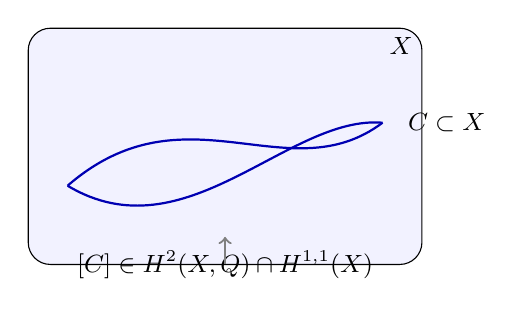
\begin{tikzpicture}[
  surface/.style={draw, fill=blue!5, minimum width=5cm, minimum height=3cm, rounded corners=8pt},
  curve/.style={thick, blue!70!black},
  label/.style={font=\small},
  arr/.style={->, thick, gray}
]
  \node[surface] (S) at (0,0) {};
  \node[font=\small, anchor=north east] at (S.north east) {$X$};

  \draw[curve] (-2,-0.5) .. controls (-0.5,0.8) and (0.8,-0.6) .. (2,0.3);
  \draw[curve] (-2,-0.5) .. controls (-0.5,-1.4) and (0.8,0.4) .. (2,0.3);

  \node[label, anchor=west] at (2.2,0.3) {$C \subset X$};
  \node[label, anchor=south] at (0,-1.8) {$[C] \in H^2(X,\mathbb{Q}) \cap H^{1,1}(X)$};

  \draw[arr] (0,-1.5) -- (0,-1.15);
\end{tikzpicture}
\caption{An algebraic curve $C$ on a surface $X$ defines a cohomology class $[C]$ of type $(1,1)$. The Hodge conjecture asserts that every rational $(p,p)$-class arises from such algebraic cycles.}
\label{fig:algebraic-cycle}
\end{figure}

\begin{theorem}[Lefschetz, 1924]
The map $\operatorname{Pic}(X) \to H^2(X, \mathbb{Z})$ sending a line bundle to its first Chern class is an isomorphism onto $H^2(X, \mathbb{Z}) \cap H^{1,1}(X)$.
\end{theorem}

This theorem is the $(1,1)$ case of the Hodge conjecture. It says that every integral $(1,1)$-class is algebraic (comes from a divisor). We will state and discuss it more carefully in Section~\ref{sec:statement}.

\begin{example}
On $\mathbb{P}^n(\mathbb{C})$, every line bundle is of the form $\mathcal{O}(d)$ for some $d \in \mathbb{Z}$, and $H^2(\mathbb{P}^n(\mathbb{C}), \mathbb{Z}) \cong \mathbb{Z}$, generated by the hyperplane class $h = c_1(\mathcal{O}(1))$. So every $(1,1)$-class is a multiple of $h$, and is algebraic.
\end{example}

\begin{example}
On an elliptic curve $E$, $\operatorname{Pic}(E) \cong \mathbb{Z} \oplus E(\mathbb{C})$, where the $\mathbb{Z}$ part corresponds to the degree and the $E(\mathbb{C})$ part to the Jacobian. The first Chern class map sends a divisor of degree $d$ to $d$ times the fundamental class of $H^2(E, \mathbb{Z}) \cong \mathbb{Z}$.
\end{example}

\section{Statement of the Hodge Conjecture}
\label{sec:statement}

\subsection{Hodge Classes}

We now have all the ingredients to state the Hodge conjecture precisely.

\begin{definition}
Let $X$ be a smooth projective variety of complex dimension $n$. A class $\alpha \in H^{2p}(X, \mathbb{Q})$ is a \emph{Hodge class} if its image under the Hodge decomposition lies in $H^{p,p}(X)$, i.e., $\alpha \in H^{2p}(X, \mathbb{Q}) \cap H^{p,p}(X)$.
\end{definition}

The space of Hodge classes is
\[
\operatorname{Hdg}^{2p}(X, \mathbb{Q}) = H^{2p}(X, \mathbb{Q}) \cap H^{p,p}(X).
\]
The cycle class map gives an injection
\[
Z^p(X)_{\mathbb{Q}} / \sim \hookrightarrow \operatorname{Hdg}^{2p}(X, \mathbb{Q})
\]
where $\sim$ denotes algebraic equivalence. The Hodge conjecture predicts that this map is surjective.

\subsection{The Conjecture}

\begin{conjecture}[Hodge, 1950]
\label{conj:hodge}
Let $X$ be a smooth projective variety over $\mathbb{C}$ of complex dimension $n$. For every $0 \le p \le n$, the cycle class map
\[
\operatorname{cl}: Z^p(X)_{\mathbb{Q}} \to H^{2p}(X, \mathbb{Q}) \cap H^{p,p}(X)
\]
is surjective. Equivalently, every rational cohomology class of type $(p,p)$ on $X$ is a $\mathbb{Q}$-linear combination of classes of algebraic cycles.
\end{conjecture}

In symbols:
\[
\operatorname{Hdg}^{2p}(X, \mathbb{Q}) = \operatorname{cl}(Z^p(X)_{\mathbb{Q}}).
\]

\begin{remark}
The conjecture is formulated with $\mathbb{Q}$-coefficients, not $\mathbb{Z}$-coefficients. The integral version is false (see Section~\ref{sec:integral}). Also, the conjecture does not ask for a single algebraic cycle representing a given Hodge class, but only for a $\mathbb{Q}$-linear combination of cycle classes. In other words, if $\alpha$ is a Hodge class, there exist irreducible subvarieties $V_1, \ldots, V_r$ of codimension $p$ and rational numbers $q_1, \ldots, q_r$ such that $\alpha = \sum q_i [V_i]$.
\end{remark}

\begin{checkyou}
\begin{enumerate}
\item Why is the integral Hodge conjecture (with $\mathbb{Z}$-coefficients) false, while the rational version (with $\mathbb{Q}$-coefficients) is expected to be true?
\item What role does torsion play in the failure of the integral conjecture?
\end{enumerate}
\end{checkyou}

\subsection{The Lefschetz $(1,1)$ Theorem}

The most important positive result is the case $p = 1$ of the Hodge conjecture.

\begin{theorem}[Lefschetz $(1,1)$ theorem]
\label{thm:lef11}
Let $X$ be a smooth projective variety over $\mathbb{C}$. Every Hodge class $\alpha \in H^2(X, \mathbb{Q}) \cap H^{1,1}(X)$ is the class of a divisor (a linear combination of codimension-1 subvarieties) with rational coefficients.
\end{theorem}

Equivalently, the Lefschetz $(1,1)$ theorem says that the Hodge conjecture is true for $p = 1$.

\begin{proof}[Proof sketch]
The proof proceeds in several steps.

\emph{Step 1: Reduction to integral classes.} Since $H^2(X, \mathbb{Q}) \cap H^{1,1}(X)$ is spanned by integral classes (classes in $H^2(X, \mathbb{Z}) \cap H^{1,1}(X)$), it suffices to prove that every integral $(1,1)$-class is the class of a divisor.

\emph{Step 2: Line bundles and divisors.} By the exponential exact sequence on $X$,
\[
0 \to \mathbb{Z} \to \mathcal{O}_X \xrightarrow{\exp(2\pi i \,\cdot)} \mathcal{O}_X^* \to 0,
\]
there is a long exact sequence in cohomology:
\[
H^1(X, \mathcal{O}_X^*) \to H^2(X, \mathbb{Z}) \to H^2(X, \mathcal{O}_X).
\]
The map $H^1(X, \mathcal{O}_X^*) \cong \operatorname{Pic}(X)$ sends a line bundle to its first Chern class in $H^2(X, \mathbb{Z})$.

\emph{Step 3: The Hodge decomposition at the level of sheaf cohomology.} By Hodge theory, the map $H^2(X, \mathbb{Z}) \to H^2(X, \mathcal{O}_X)$ factors through the projection onto $H^{0,2}(X)$ in the Hodge decomposition. By complex conjugation symmetry, $h^{0,2} = h^{2,0}$. The kernel of $H^2(X, \mathbb{Z}) \to H^2(X, \mathcal{O}_X)$ is exactly $H^2(X, \mathbb{Z}) \cap (H^{2,0}(X) \oplus H^{1,1}(X))$. But since $H^2(X, \mathbb{Z})$ consists of integral classes, and the projection to $H^{2,0}$ is injective on $H^2(X, \mathbb{Z})$ (by the Hodge decomposition), the kernel of the map to $H^2(X, \mathcal{O}_X)$ is $H^2(X, \mathbb{Z}) \cap H^{1,1}(X)$.

Wait, let me be more precise. The image of $H^2(X, \mathbb{Z})$ in $H^2(X, \mathcal{O}_X) \cong H^{0,2}(X)$ is the projection of integral classes onto the $(0,2)$-part. An integral class $\alpha \in H^2(X, \mathbb{Z})$ maps to zero in $H^{0,2}(X)$ if and only if $\alpha$ has no $(0,2)$-component, i.e., $\alpha$ lies in $H^{2,0}(X) \oplus H^{1,1}(X)$. But since $\alpha = \bar{\alpha}$ (as an integral class), the $(2,0)$-component is the conjugate of the $(0,2)$-component, so if the $(0,2)$-component is zero, so is the $(2,0)$-component. Therefore, $\alpha$ lies in $H^{1,1}(X)$.

Conversely, if $\alpha \in H^2(X, \mathbb{Z}) \cap H^{1,1}(X)$, then $\alpha$ has zero $(2,0)$- and $(0,2)$-components, so it maps to zero in $H^2(X, \mathcal{O}_X)$.

Thus $H^2(X, \mathbb{Z}) \cap H^{1,1}(X) = \ker(H^2(X, \mathbb{Z}) \to H^2(X, \mathcal{O}_X))$.

\emph{Step 4: From the exact sequence.} The exact sequence of Step 2 shows that the kernel of $H^2(X, \mathbb{Z}) \to H^2(X, \mathcal{O}_X)$ is the image of $\operatorname{Pic}(X) \to H^2(X, \mathbb{Z})$. So every integral $(1,1)$-class comes from a line bundle. Since every line bundle on a smooth projective variety is isomorphic to $\mathcal{O}(D)$ for some divisor $D$ (by the divisor associated to a global section), the class comes from a divisor.

Actually, the last step needs more care. Not every line bundle has a global section. But on a smooth projective variety, every line bundle is a difference of line bundles with sections (by taking powers). More precisely, if $L$ is a line bundle with $c_1(L) \in H^2(X, \mathbb{Z}) \cap H^{1,1}(X)$, then $L$ maps to zero in $H^2(X, \mathcal{O}_X)$, so $L$ is in the image of $\operatorname{Pic}(X) \to H^2(X, \mathbb{Z})$. By the exact sequence, $L = \mathcal{O}(D)$ for some Weil divisor $D$ on $X$ (which on a smooth variety is the same as a Cartier divisor). The class of $D$ in $H^2(X, \mathbb{Z})$ is $c_1(\mathcal{O}(D)) = c_1(L)$.
\end{proof}

\begin{remark}
The Lefschetz $(1,1)$ theorem is a special case of the Lefschetz theorem on $(1,1)$-classes, which is part of the more general theory of Lefschetz hyperplane theorems. It was proved by Lefschetz in 1924, well before Hodge formulated his conjecture.
\end{remark}

\begin{checkyou}
\begin{enumerate}
\item Why is the Lefschetz $(1,1)$ theorem easier than the full Hodge conjecture? What extra structure does codimension~1 have that higher codimensions lack?
\item The proof uses the exponential exact sequence. Why is there no analogous exact sequence for $p \ge 2$?
\end{enumerate}
\end{checkyou}

\subsection{Why $p = 1$ Is Solved and Higher $p$ Is Not}

The Lefschetz $(1,1)$ theorem works because of the exact sequence of the exponential sheaf, which provides a direct link between line bundles (algebraic objects) and $H^2$-cohomology (topological objects). For higher $p$, there is no analogous exact sequence. The higher-codimensional analogues of line bundles are \emph{vector bundles} of rank $> 1$, and the relationship between vector bundles and cohomology is governed by Chern classes, which land in $H^{2k}(X, \mathbb{Z})$ for $k \le \operatorname{rank}(E)$. These Chern classes do not, in general, generate all of $H^{2p}(X, \mathbb{Z}) \cap H^{p,p}(X)$ for $p \ge 2$.

Another way to see the difficulty: for $p = 1$, a divisor on a smooth variety is determined (up to linear equivalence) by its line bundle, and line bundles are classified by $H^1(X, \mathcal{O}_X^*)$, which is related to $H^2(X, \mathbb{Z})$ by the exponential exact sequence. For $p \ge 2$, algebraic $p$-cycles are classified by Chow groups $A^p(X)$, which are much more mysterious and generally infinite-dimensional (not finitely generated as abelian groups, in contrast to cohomology groups).

\subsection{Status for General $p$}

For $p \ge 2$, the Hodge conjecture is open in general. The conjecture is expected to be true (i.e., there are no known counterexamples for smooth projective varieties), but the known cases are limited to:
\begin{itemize}
\item Varieties of dimension $\le 2$ (trivially).
\item The Lefschetz $(1,1)$ theorem (all codimension 1).
\item Certain special classes of varieties (abelian varieties, K3 surfaces, etc.).
\item Certain special degrees (e.g., $2p = \dim X$ by the Hard Lefschetz theorem and the theory of Hodge structures).
\end{itemize}

\section{What Is Known}
\label{sec:known}

\subsection{The Lefschetz $(1,1)$ Theorem}

As we proved in Section~\ref{sec:statement}, the Lefschetz $(1,1)$ theorem establishes the Hodge conjecture for $p = 1$: every Hodge class in $H^2(X, \mathbb{Q}) \cap H^{1,1}(X)$ is algebraic.

\begin{corollary}
The Hodge conjecture holds for divisors on any smooth projective variety.
\end{corollary}

\subsection{Curves and Surfaces}

For varieties of dimension $\le 2$, the Hodge conjecture is true (though this is not very deep).

\begin{proposition}
Let $X$ be a smooth projective curve ($\dim X = 1$). Then the Hodge conjecture holds for $X$.
\end{proposition}

\begin{proof}
For a curve, $H^0(X, \mathbb{Q}) \cong \mathbb{Q}$ is generated by the fundamental class (the constant function), which is algebraic. $H^2(X, \mathbb{Q}) \cong \mathbb{Q}$ is generated by the class of a point, which is algebraic. There are no $H^1$ classes of type $(p,p)$ (since $p + q = 1$ implies $p \neq q$). So the Hodge conjecture holds trivially.
\end{proof}

\begin{proposition}
Let $X$ be a smooth projective surface ($\dim X = 2$). Then the Hodge conjecture holds for $X$.
\end{proposition}

\begin{proof}
The relevant cohomology groups are:
\begin{itemize}
\item $H^0(X, \mathbb{Q}) \cong \mathbb{Q}$: generated by the fundamental class, algebraic.
\item $H^1(X, \mathbb{Q})$: no $(p,p)$-classes (since $p + q = 1$ implies $p \neq q$).
\item $H^2(X, \mathbb{Q})$: this is $H^{2,0} \oplus H^{1,1} \oplus H^{0,2}$. The Hodge classes are $H^2(X, \mathbb{Q}) \cap H^{1,1}(X)$, and by the Lefschetz $(1,1)$ theorem, every such class is algebraic.
\item $H^3(X, \mathbb{Q})$: no $(p,p)$-classes (since $p + q = 3$ implies $p \neq q$).
\item $H^4(X, \mathbb{Q}) \cong \mathbb{Q}$: generated by the class of a point, algebraic.
\end{itemize}
So the Hodge conjecture holds for surfaces.
\end{proof}

\subsection{Abelian Varieties}

An abelian variety $A$ of dimension $g$ is a complex torus $\mathbb{C}^g / \Lambda$ that admits a K\"{a}hler metric (and hence is algebraic). The Hodge structure of $A$ is particularly tractable because $A$ is a product of one-dimensional tori at the level of cohomology.

\begin{theorem}
The Hodge conjecture holds for abelian varieties in the following cases:
\begin{enumerate}
\item For products of elliptic curves with complex multiplication.
\item For abelian varieties of dimension $\le 3$ (partial results).
\item For certain classes of abelian varieties determined by their Mumford--Tate groups.
\end{enumerate}
\end{theorem}

The general case is open. The key tool is the theory of Mumford--Tate groups, which controls the Hodge structure on the cohomology of an abelian variety. If the Mumford--Tate group is small (e.g., for abelian varieties with many endomorphisms), the Hodge conjecture can be verified. For ``generic'' abelian varieties, the Mumford--Tate group is as large as possible (the full symplectic group), and less is known.

\begin{example}
Let $E_1, E_2$ be two elliptic curves. The product $A = E_1 \times E_2$ is an abelian surface (dimension 2). The Hodge conjecture holds for $A$ by the dimension $\le 2$ argument. But the Hodge conjecture for abelian varieties of dimension 3 (products of three elliptic curves) already requires deeper input.
\end{example}

\subsection{K3 Surfaces}

The Hodge conjecture for K3 surfaces was proved in the 1980s by several authors.

\begin{theorem}[van der Geer, Looijenga, Piatetski-Shapiro, Siu]
Let $X$ be a K3 surface. Then every Hodge class on $X$ is algebraic: $H^2(X, \mathbb{Q}) \cap H^{1,1}(X)$ is generated by classes of algebraic curves.
\end{theorem}

\begin{remark}
The proof uses the fact that on a K3 surface, $h^{2,0} = 1$ and $h^{1,1} = 20$. The 20-dimensional space $H^{1,1}(X) \cap H^2(X, \mathbb{Q})$ is generated by the classes of algebraic curves and the class of the K\"{a}hler form. The algebraic curves are ample divisors, and their classes span $H^{1,1} \cap H^2(X, \mathbb{Q})$ by a lattice-theoretic argument (using the fact that the N\'eron--Severi group has rank $\rho = h^{1,1} = 20$ for a K3 surface with maximal Picard number, and the fact that for a general K3 surface, $\rho = 1$, but the Hodge conjecture still holds).
\end{remark}

\subsection{The Integral Hodge Conjecture}
\label{sec:integral}

The integral Hodge conjecture asks whether the cycle class map
\[
\operatorname{cl}: Z^p(X) \to H^{2p}(X, \mathbb{Z}) \cap H^{p,p}(X)
\]
is surjective (with integer, rather than rational, coefficients).

\begin{theorem}[Atiyah--Hirzebruch, 1962]
The integral Hodge conjecture is false in general. There exist smooth projective varieties $X$ and classes $\alpha \in H^{2p}(X, \mathbb{Z}) \cap H^{p,p}(X)$ that are not the class of an integral algebraic cycle.
\end{theorem}

The counterexample uses a four-dimensional manifold $X$ constructed as a fibration, with $H^4(X, \mathbb{Z}) \cap H^{2,2}(X)$ containing a class that is not algebraic. The key point is that the cycle class map, with integer coefficients, is not surjective: there are torsion phenomena and other obstructions that do not appear with rational coefficients.

\begin{remark}
This is why the Hodge conjecture is formulated with $\mathbb{Q}$-coefficients. The passage to rational coefficients kills the torsion and makes the conjecture plausible. The integral version is a strictly stronger statement, and it fails.
\end{remark}

\subsection{Further Partial Results}

Beyond the cases discussed above, the Hodge conjecture has been verified in several other special situations:

\begin{itemize}
\item \textbf{Grassmannians and flag varieties:} The cohomology of Grassmannians is generated by Schubert cycles, which are algebraic. So the Hodge conjecture holds for all Grassmannians.
\item \textbf{Complete intersections:} For certain complete intersections in projective space, the Hodge conjecture is known (e.g., for cubic fourfolds, by work of Voisin and others, though the full conjecture is open).
\item \textbf{Motives and the standard conjectures:} The Hodge conjecture is closely related to the standard conjectures of Grothendieck, which concern the algebraicity of certain correspondence classes. If the standard conjectures hold, then the Hodge conjecture would follow in many cases.
\item \textbf{The generalized Hodge conjecture:} Grothendieck formulated a generalization of the Hodge conjecture involving mixed Hodge structures. This generalization is also open.
\end{itemize}

\subsection{The Relationship to Other Millennium Problems}

The Hodge conjecture has connections to several other Millennium Prize Problems:

\begin{itemize}
\item \textbf{Poincar\'{e} conjecture (now theorem):} The Hodge conjecture is not directly related to the Poincar\'{e} conjecture, but both concern the relationship between topology and geometry.
\item \textbf{Birch and Swinnerton-Dyer conjecture:} The BSD conjecture relates the rank of an elliptic curve to the order of vanishing of its $L$-function. The Hodge conjecture provides the cohomological framework for understanding algebraic cycles on elliptic curves and abelian varieties.
\item \textbf{Riemann hypothesis:} The Riemann hypothesis for varieties over finite fields (proved by Deligne) uses the theory of Hodge structures and the Weil conjectures, which are related to the Hodge conjecture.
\end{itemize}

\section{Exercises}

\begin{exercise}
Compute the Hodge diamond of $\mathbb{P}^3(\mathbb{C})$. What are the Betti numbers $b_k$ for $0 \le k \le 6$?
\end{exercise}

\begin{exercise}
Let $C \subset \mathbb{P}^2(\mathbb{C})$ be a smooth curve of degree $d$. Using the formula $g = \frac{(d-1)(d-2)}{2}$ for the genus, compute the Hodge numbers $h^{1,0}$ and $h^{0,1}$ of $C$. Verify that $b_1(C) = 2g$.
\end{exercise}

\begin{exercise}
Let $X \subset \mathbb{P}^3(\mathbb{C})$ be a smooth surface of degree $d$. Compute the Euler characteristic $\chi(X) = 2 - 2b_1 + b_2$ and express it in terms of $d$. (Hint: Use the fact that $b_1 = 0$ for a hypersurface in $\mathbb{P}^3$ and compute $b_2$ from the degree and the genus of hyperplane sections.)
\end{exercise}

\begin{exercise}
Verify the Hodge decomposition for the 2-torus $T^2 = S^1 \times S^1$. Compute $H^{1,0}(T^2)$ and $H^{0,1}(T^2)$ and show that $h^{1,0} = h^{0,1} = 1$.
\end{exercise}

\begin{exercise}
Let $X$ be a smooth projective variety of dimension $n$. Prove that $h^{n,n} = 1$ (i.e., $H^{n,n}(X, \mathbb{C}) \cong \mathbb{C}$). Interpret this in terms of the fundamental class of $X$.
\end{exercise}

\begin{exercise}
Show that on a K3 surface $X$, every class in $H^2(X, \mathbb{Q}) \cap H^{1,1}(X)$ is a multiple of the hyperplane class if and only if the Picard number $\rho(X) = 1$. For a general K3 surface, what is $\rho(X)$?
\end{exercise}

\begin{exercise}
Let $E_1, E_2$ be elliptic curves and $X = E_1 \times E_2$. Compute the Hodge diamond of $X$. Identify all Hodge classes in $H^2(X, \mathbb{Q})$ and show that they are all algebraic (generated by classes of curves of the form $E_1 \times \{p\}$ and $\{p\} \times E_2$).
\end{exercise}

\begin{exercise}
The Fermat quintic threefold $X_5 \subset \mathbb{P}^4(\mathbb{C})$ defined by $x_0^5 + x_1^5 + x_2^5 + x_3^5 + x_4^5 = 0$ has Hodge numbers $h^{1,1} = 1$ and $h^{2,1} = 101$. Explain why the Hodge conjecture for $X_5$ reduces to showing that every $(1,1)$-class is algebraic (which is true by the Lefschetz $(1,1)$ theorem). Are there Hodge classes in $H^4(X_5, \mathbb{Q}) \cap H^{2,2}(X_5)$? Why or why not?
\end{exercise}

\begin{exercise}
Show that the cycle class map $\operatorname{cl}: Z^1(X)_{\mathbb{Q}} \to H^2(X, \mathbb{Q}) \cap H^{1,1}(X)$ is not injective in general: there exist nontrivial divisors that are homologous to zero. (Hint: Consider linearly equivalent divisors on a curve.)
\end{exercise}

\begin{exercise}
Let $X$ be a smooth projective surface. Show that $H^4(X, \mathbb{Q}) \cap H^{2,2}(X) = H^4(X, \mathbb{Q})$ (all classes in $H^4$ are of type $(2,2)$). Conclude that the Hodge conjecture for $H^4$ on a surface is equivalent to saying that the class of a point is algebraic. Verify this directly.
\end{exercise}

\begin{exercise}
Let $A$ be an abelian variety of dimension $g$. Using the fact that $A \cong \mathbb{C}^g / \Lambda$ and the Künneth formula, show that the Hodge diamond of $A$ is the $g$-fold tensor product of the Hodge diamond of an elliptic curve. Compute $h^{1,0}(A)$ and $h^{0,1}(A)$.
\end{exercise}

\begin{exercise}
\textbf{Challenge.} The integral Hodge conjecture for 4-folds is false by the Atiyah--Hirzebruch theorem. Explain why the failure of the integral conjecture does not contradict the rational Hodge conjecture. Give an explicit example of a torsion class in $H^4(X, \mathbb{Z})$ that is not the class of an integral algebraic cycle, but becomes algebraic after tensoring with $\mathbb{Q}$. (Hint: Consider a smooth hypersurface of degree 6 in $\mathbb{P}^5(\mathbb{C})$, which is a 4-fold.)
\end{exercise}

\section{Further Reading}

\begin{itemize}
\item P. Deligne, ``The Hodge conjecture,'' in \textit{Mathematics: Frontiers and Perspectives}, AMS, 2000. The official Clay Mathematics Institute problem description.
\item C. Voisin, \textit{Hodge Theory and Complex Algebraic Geometry}, Vols.\ I and II, Cambridge University Press, 2003. A comprehensive modern treatment.
\item J.\ D.\ Lewis, \textit{A Survey of the Hodge Conjecture}, AMS, 1999. A detailed survey of the state of the art.
\item W.\ V.\ D.\ Hodge, \textit{The Theory and Applications of Harmonic Integrals}, Cambridge University Press, 1941. The original work introducing Hodge theory.
\item R.\ L.\ Bott and L.\ W.\ Tu, \textit{Differential Forms in Algebraic Topology}, Springer, 1982. An excellent introduction to de Rham cohomology and spectral sequences.
\item D.\ Mumford, \textit{Algebraic Geometry I: Complex Projective Varieties}, Springer, 1976. A concise introduction to the algebraic geometry underlying the Hodge conjecture.
\end{itemize}

\section*{Chapter Summary}

\noindent\textbf{What we learned:}
\begin{itemize}
  \item A \emph{K\"{a}hler manifold} has compatible complex, symplectic, and Riemannian structures, forcing strong topological constraints.
  \item The \emph{Hodge decomposition} splits $H^k(X, \mathbb{C}) = \bigoplus_{p+q=k} H^{p,q}(X)$ into types, with symmetries $h^{p,q} = h^{q,p}$ and $h^{p,q} = h^{n-p,n-q}$.
  \item A \emph{Hodge class} is a rational cohomology class of type $(p,p)$. The Hodge conjecture says all Hodge classes are algebraic (combinations of subvariety classes).
  \item The \emph{Lefschetz $(1,1)$ theorem} proves the conjecture for codimension 1: every $(1,1)$-class on a smooth projective variety is algebraic.
  \item The conjecture is known for curves and surfaces, and for certain special classes (abelian varieties, Fermat varieties), but open in general.
\end{itemize}

\noindent\textbf{Key technique:} Hodge theory---using harmonic forms and the Laplacian on a K\"{a}hler manifold to decompose cohomology into types, connecting topology to complex geometry.

\noindent\textbf{Connections to other chapters:} The Hodge decomposition uses the same Laplacian that appears in the heat equation and Navier--Stokes (Chapter~4). The cycle class map connects algebraic geometry to topology, relating to the Birch--Swinnerton-Dyer conjecture (Chapter~7) through the theory of elliptic curves.
